\documentclass[twoside,english]{uiofysmaster}
%\bibliography{references}

\usepackage{array}
\usepackage{booktabs}
\usepackage{float}
\usepackage{scrextend}
\usepackage{amsfonts}
\usepackage{amsmath,amsfonts,amssymb}
\addtokomafont{labelinglabel}{\sffamily}

\usepackage[boxed]{algorithm2e}
\addtokomafont{labelinglabel}{\sffamily}

% Feynman slash
\usepackage{slashed}

% To show code
\usepackage{listings}

% For quotes
\usepackage[autostyle]{csquotes} 

% For subfigures
\usepackage{subcaption}

\setlength{\heavyrulewidth}{1.5pt}
\setlength{\abovetopsep}{4pt}

\begin{document}

\tableofcontents



\chapter{Gaussian Processes}

In this chapter Gaussian process regression is introduced and explained. To begin with some concepts and expressions in Bayesian statistics are introduced. The following section introduces the mathematical framework needed, before some covariance functions are discussed. A few concepts in Bayesian model selection are used as a basis to quantify the quality of predictions. Finally, distributed Gaussian processes are introduced as a way of scaling Gaussian processes to larger datasets.

\section{Introduction to Bayesian Statistics}

As it turns out, statistics are not merely statistics. In fact, there is great disagreement between the \textit{frequentist} statisticians and the \textit{Bayesian} statisticians as to what statistics should be . In order to understand the dispute, first consider a statement they \textit{do} agree on

\begin{center}
\textit{Statisticians use probability to describe uncertainty.}
\end{center}

This seems reasonable. Where statisticians reach disagreement is at the definition of the \textit{uncertain}. Defining the uncertain defines probability, and one can distinguish between two branches, namely \textit{objective} and \textit{subjective} probability. Consider an example in which a statistician throws a dice. Before throwing, he is uncertain about the outcome of the dice toss. This uncertainty related to the outcome is \textit{objective}: no one can know if he will throw a 1 or a 4. On the other hand, he might also be uncertain about the underlying probability distribution of the dice toss. Is the dice loaded? Is one of the edges sharper than the others? This uncertainty is \textit{subjective}, as it may vary from person to person depending on how much information one has about the system. One of the main critiques of subjective probability posed by frequentists is that the final probability depends on who you ask.

\subsection{Bayes' Theorem}

To further illustrate the difference a soundingly Bayesian framework is introduced, namely \textit{Bayes' theorem}. Bayes' theorem can be derived from the familiar rules of probability
\begin{align}\label{Eq:: Sum rule}
P(X | I) + P(\bar{X} | I) = 1,
\end{align}
\begin{align}\label{Eq:: Product rule}
P(X, Y | I) = P(X | Y, I) \times P(Y | I),
\end{align} 
commonly known as the \textit{sum rule} and \textit{product rule}, respectively. $P(X|I)$ means the probability of outcome $X$ given the information $I$, and $P(X|Y,I)$ means the probability of outcome $X$ given the information $I$ \textit{and} outcome $Y$. The bar over $\bar{X}$ means that the outcome $X$ does \textit{not} happen. The sum rule states that the probability of the outcome $X$ happening plus the probability of $X$ not happening is equal to 1. This is rather untuitive, considering an event either takes place or it doesn't. The second rule, the product rule, states that the probability of both outcomes $X$ and $Y$ is equal to the probability of $Y$ times the probability of $X$ given that $Y$ has already happened. 
These expressions can easily be combined into Bayes' theorem, first formulated by reverend Thomas Bayes in 1763,
\begin{align}\label{Eq:: gaussian process : Bayes theorem}
P(X | Y, I) = \frac{P(Y | X, I) \times P(X | I)}{P(Y | I)}.
\end{align}
This theorem states that the probability of $X$ given $Y$ equals the probability of $Y$ given $X$ times the probability of $X$, divided by the probability of $Y$. So what is Bayesian about Bayes' theorem? \textit{Nothing}. It merely reformulates the rules of logical consistent reasoning stated by Richard Cox in 1946 \cite{sivia2006data}. Laplace was the one to make Bayes' theorem Bayesian, when he used the theorem to perform inference about distribution parameters. These are, for example, the mean and variance of a Gaussian distribution. The resulting expression is
\begin{align}
P(\Theta = \theta | X=x) = \frac{P(X=x|\Theta = \theta) P(\Theta = \theta)}{P(X=x)},\label{Eq:: gaussian process : Bayesian inference}
\end{align}
where $\Theta$ are the possible probability distribution parameters, $X$ are the possible outcomes, $P(X=x)$ is a normalization constant called the \textit{marginal likelihood}, and $P(X=x|\Theta = \theta)$  and $P(\Theta = \theta)$ are the \textit{likelihood} and \textit{prior}, respectively, both of which will be revisited later. In other words, Eq. (\ref{Eq:: gaussian process : Bayesian inference}) states the probability of the parameters $\theta$, given the knowledge of outcomes $x$.

A crucial parting of the Bayesians from the frequentists is at the introduction of the \textit{prior}, which expresses a probability distribution on the \textit{parameters} of the probability distribution. Fret not, this will be further explained.

\subsection{Priors and Likelihood}

The likelihood $P(X = x |\Theta = \theta)$ is simply the probability of the observations given the parameters. The prior, on the other hand, expresses a prior belief or assumption of the data, and has to be determined beforehand. The measure $P(\Theta = \theta | X = x)$ from Eq. (\ref{Eq:: gaussian process : Bayesian inference}) is called the \textit{posterior distribution}. This can be thought of as the prior belief, modified by how well this belief fits the data,
\begin{align*}
\text{posterior} = \frac{\text{prior} \times \text{likelihood}}{\text{marginal likelihood}}.
\end{align*}
Consider an example. The statistician from before has now grown tired of throwing dice, and starts to throw a coin. Before throwing he assumes the probability of getting heads or tails is equal, and so adopts a flat prior. After one throw he gets heads, and the posterior changes to a function with high probability for heads, and low for tails. Another heads makes the posterior even narrower around 1, but after several throws the distribution converges to a narrow peak around $0.25$, as can be seen in Fig. (\ref{Fig:: gaussian process : Dice throw }), along with other examples of priors. This indicates an unfair coin. Note that the different priors arrive at the same posterior after a large amount of throws.

\begin{figure}
\centering
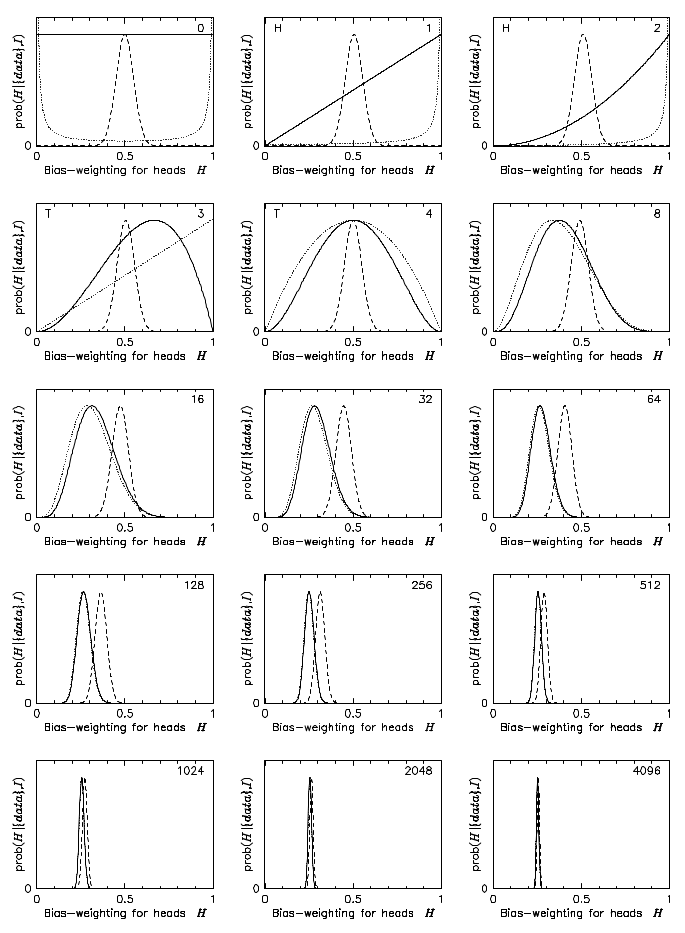
\includegraphics[scale=0.65]{sivia_coin_toss.png}
\caption{The effect of different priors, $P(H|I)$, on the posterior pdf for the bias-weighting of a coin. The solid line is a flat prior, the dashed line assumes a fair coin, and the dotted line is the Jeffreys prior. Figure from \cite{sivia2006data}.}
\label{Fig:: gaussian process : Dice throw }
\end{figure}


\subsection{Best Estimate and Reliability}

Now that the posterior distribution has been defined, it would be useful to quantify how well it actually fits the data. For that purpose the \textit{best estimate} and \textit{reliability} are introduced. The best estimate $X_0$  is the outcome with the highest probability. In other words, it is the maximum of the posterior
\begin{align}
&\frac{dP}{dX}\Big|_{X_0} = 0, &\frac{d^2P}{dX^2}\Big|_{X_0} < 0.
\end{align}
The second derivative must be negative in order to insure that it is, in fact, a maximum. Once the best estimate has been found, one should ask oneself how reliable this estimate is. Reliability is represented by the width of the distribution, or how much the data is smeared out. A very narrow distribution has very low uncertainty, while a wide distribution has large uncertainty. The width is found using a Taylor expansion of the posterior, and taking the logarithm \footnote{$L$ is a monotonic function of $P$, so the maximum of $L$ is at the maximum of $P$.}
\begin{align}
&L = L(X_0) + \frac{1}{2} \frac{d^2}{dx^2} L\Big|_{X_0} (X-X_0)^2 +... ,&L = \log_e \Big[\text{prob}(x | \{data\}, I) \Big]\label{Eq:: gaussian process : Taylor expansion L}
\end{align}
This gives a proximate posterior which is a \textit{Gaussian distribution}, with mean and variance given by
\begin{align}
&\mathcal{N}( \mu, \sigma) \text{ where } \mu = X_0\text{, } \sigma = \Big( - \frac{d^2L}{dx^2} \Big)^{-1/2}.
\end{align}
The Gaussian distribution is symmetric with respect to the maximum at $x = \mu$, and has a full width at half maximum (FWHM) at around $2.35 \sigma$, as shown in Fig. (\ref{Fig:: gaussian process : Gaussian distribution}).

\begin{figure}
\centering
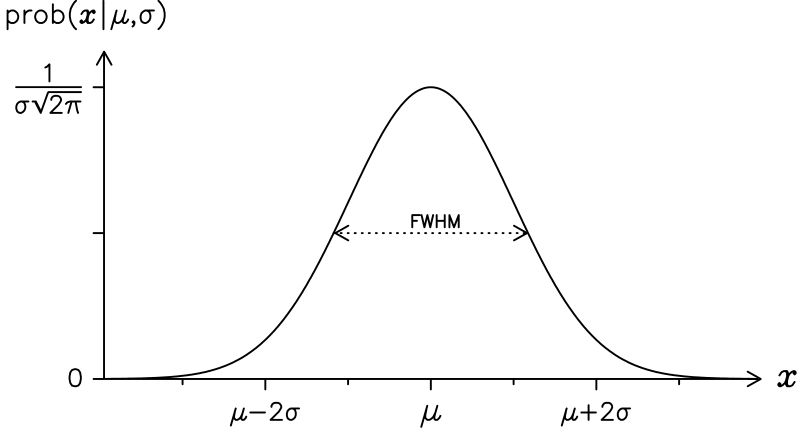
\includegraphics[scale=0.5]{sivia_gaussian_distribution.png}
\caption{A Gaussian probability distribution. The maximum is at the mean value $\mu$, with a full width at half maximum (FWHM) at around $2.35 \sigma$. Figure from \cite{sivia2006data}.}
\label{Fig:: gaussian process : Gaussian distribution}
\end{figure}

\subsection{Covariance}

The final term needed before embarking on Gaussian processes is \textit{covariance}. Covariance is discussed in more detail in \cite{sivia2006data}, a brief summary is given here. In most cases the expressions one has to solve are not as simple as Eq. (\ref{Eq:: gaussian process : Taylor expansion L}), as the probability distribution will normally have several quantities of interest $\{ X_i \}$. In that case, one has to solve a set of \textit{simultaneous equations} in order to get the best estimate
\begin{align}\label{Eq:: gaussian process : Best estimate X_i}
\frac{dP}{dX_i} \Big|_{X_{0j}} =0.
\end{align}
As a simple example consider the problem in two dimensions, so that $\{ X_i \} = (X, Y)$. The Taylor expansion of $L$ is then
\begin{align}\label{Eq:: gaussian process : Taylor expansion L_i}
L =& L(X_0, Y_0) + \frac{1}{2} \Big[ \frac{d^2L}{dX^2}  \Big|_{X_0, Y_0}(X-X_0)^2 \nonumber \\
& + \frac{d^2L}{dY^2}  \Big|_{X_0, Y_0}(Y-Y_0)^2 + 2 \frac{d^2L}{dXdY}  \Big|_{X_0, Y_0}(X-X_0)(Y-Y_0) \Big] +...
\end{align}
There are now four partial derivatives, reduced to three using the rules for mixed partial derivatives $\frac{\partial^2}{\partial X \partial Y} = \frac{\partial^2}{\partial Y \partial X}$. Writing the quadratic part of \ref{Eq:: gaussian process : Taylor expansion L_i} in matrix form gives
\begin{align}
Q = 
\begin{pmatrix}
X-X_0 & Y -Y_0
\end{pmatrix}
\begin{pmatrix}
A & C\\
C & B
\end{pmatrix}
\begin{pmatrix}
X -X_0\\
Y-Y_0
\end{pmatrix},
\end{align}
where the matrix elements are
\begin{align}
&A = \frac{\partial^2 L}{\partial X^2} \Big|_{X_0, Y_0}, &B = \frac{\partial^2 L}{\partial Y^2} \Big|_{X_0, Y_0}, &&C = \frac{\partial^2 L}{\partial X \partial Y} \Big|_{X_0, Y_0}.
\end{align}
The \textit{variance} is defined as the expectation value of the square of deviations from the mean. In the two-dimensional case this becomes \cite{sivia2006data}
\begin{align}
\text{Var}(X) = \sigma_x^2 = \braket{(X - X_0)^2} = \int \int (X - X_0)^2 P (X, Y | \{\text{data}\}, I) dXdY.
\end{align}
This is the variance $\sigma_X^2$ for $X$, and its square root is the standard deviation $\sigma_X$. A similar expression can be found for $Y$, by switching $X$ and $Y$. It is also possible to find the simultaneous deviations of the parameters $X$ and $Y$, or the correlation between the inferred parameters. This is called the \textit{covariance} $\sigma_{XY}^2$, and is in the two-dimensional case
\begin{align}
\sigma_{XY}^2 = \braket{(X - X_0) (Y - Y_0)} =\int \int (X - X_0) (Y - Y_0) P (X, Y | \{\text{data}\}, I) dXdY.
\end{align}
The covariance indicates how an over- or underestimation of one parameter affects the other parameter. If, for example, an overestimation of $X$ leads to an overestimation of $Y$, the covariance is positive. If the overestimation of $X$ has little or no effect on the estimation of $Y$, the covariance is negligible or zero $|\sigma_{XY}| \ll \sqrt{\sigma_X^2 \sigma_Y^2}$. These effects are illustrated in Fig. (\ref{Fig:: gaussian process : Covariance illustrated}). It can be shown that \cite{sivia2006data}
\begin{align}
\text{cov} = 
\begin{pmatrix}
\sigma_X^2 & \sigma_{XY}^2\\
\sigma_{XY}^2 & \sigma_Y^2
\end{pmatrix}
= - \begin{pmatrix}
A & C\\
C & B
\end{pmatrix}^{-1}.
\end{align}
This is called the \textit{covariance matrix}.

\begin{figure}
\centering
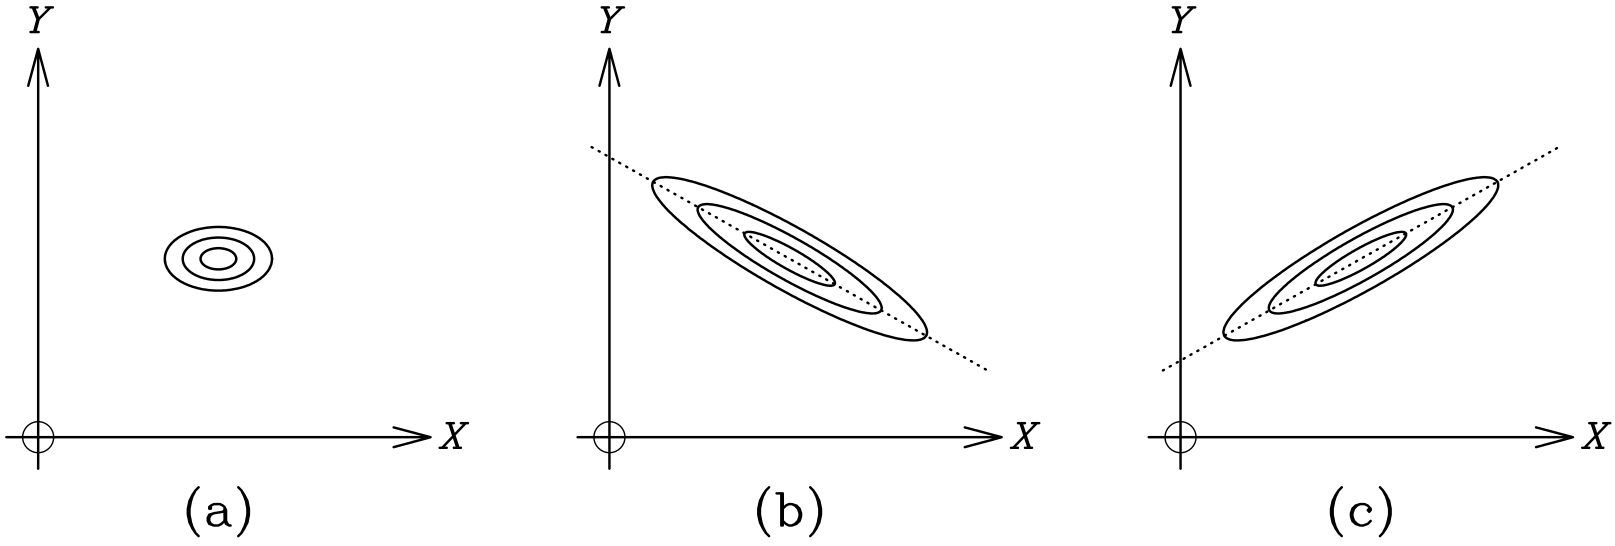
\includegraphics[scale=0.25]{sivia_covariance_correlation.png}
\caption{A schematic illustration of covariance and correlation. (a) The contours of a posterior pdf with zero covariance, where the inferred values of $X$ and $Y$ are uncorrelated. (b) The corresponding plot when the covariance is large and negative; $Y + mX =$ constant along the dotted line (where $m > 0$), emphasizing that only this sum of the two parameters can be inferred reliably. (c) The case of positive correlation, where we learn most about the difference $Y − mX$; this is constant along the dotted line. Figure from \cite{sivia2006data}}
\label{Fig:: gaussian process : Covariance illustrated}
\end{figure}


\section{Gaussian Process Regression}

Now that some basics of Bayesian statistics have been covered it is time to delve into the subject of Gaussian processes. Gaussian processes (GP) is a supervised machine learning method, designed to solve regression and probabilistic classification problems, although this thesis will only use regression. As experience dictates that Gaussian processes can be hard to grasp, it will serve both the reader and the author well to begin on a conceptual level: \textit{what do Gaussian processes do?}

Consider a set of points $\mathcal{D} = \{\textbf{x}_i, y_i\}$, where $y$ is some (possibly noisy) function of $\textbf{x}$, $y = f(\textbf{x}) + \varepsilon$. This is illustrated by the black dots in in Fig. (\ref{Fig:: gaussian process : GP illustration}). In machine learning $\mathcal{D}$ is the \textit{training data}, as it is used to train the model. It consists of \textit{features}, which are the input vectors $\textbf{x}_i$, and \textit{targets}, which are the function values $y_i$. The set of points is discrete, so there is some $\textbf{x}^*$ for which the target $y^*$ is unknown. Gaussian Processes (GP) predict a Gaussian distribution \textit{over function values} at this point $\textbf{x}^*$, with a corresponding mean $m(\textbf{x}^*)$ and variance $\sigma^2$. The GP prediction for the target value $y^*$ is the mean $m(\textbf{x}^*)$, with uncertainty $\sigma^2$. One can view the predicted target $y^*$ as a linear combination of the known targets $y_i$, where the weights are the covariances between $\textbf{x}_i$ and the test point $\textbf{x}^*$.  


\begin{figure}
\centering
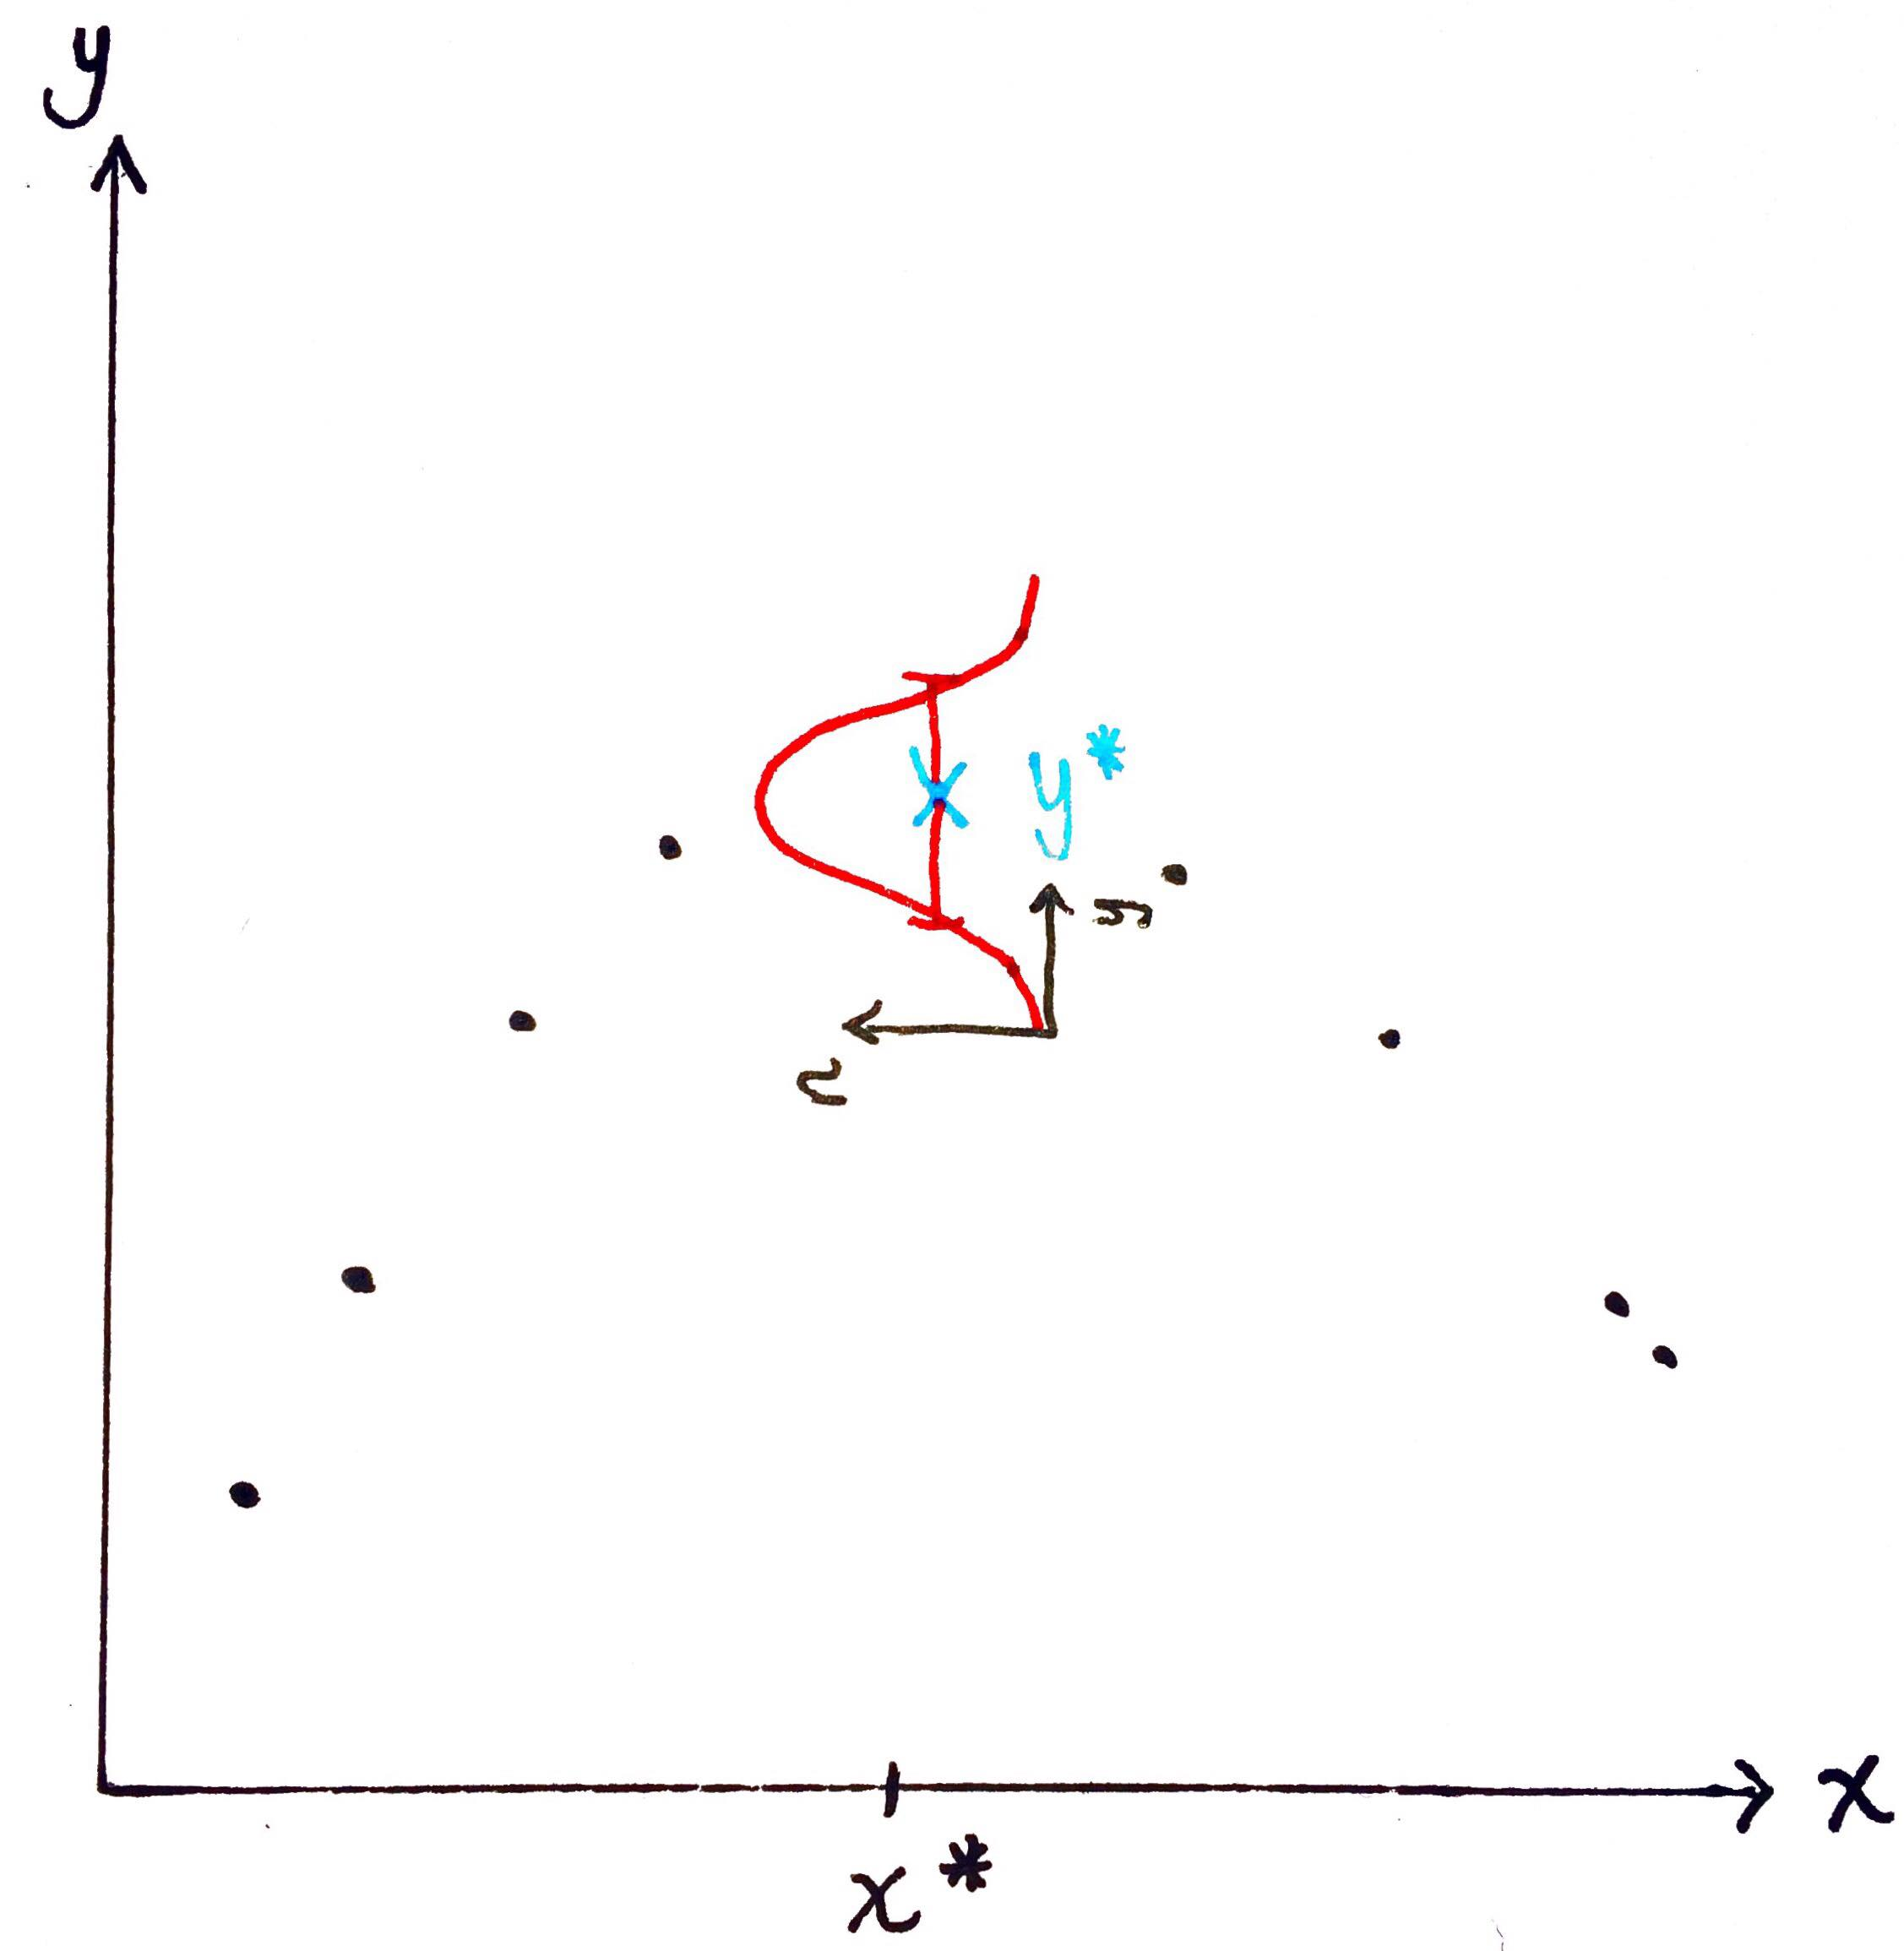
\includegraphics[scale=0.1]{GP_illustration_tegning.jpg}
\caption{An illustration of a GP prediction of the target value $y^*$ (blue cross), given the known set of points $\{x_i, y_i\}$ (black dots). The prediction is a Gaussian distribution in $y$ with mean $y^*$ and variance $\sigma^2$. The Gaussian distribution is drawn in red with $y$ on the vertical axis and the number of events $n$ on the horizontal axis, with uncertainty in the $y$-direction.}
\label{Fig:: gaussian process : GP illustration}
\end{figure}

For a real process $f(\textbf{x})$ the mean  $m(\textbf{x})$ and covariance function $k(\textbf{x}, \textbf{x}')$ are defined as
\begin{align}
m(\textbf{x}) &= \mathbb{E}[f(\textbf{x})],\\
k(\textbf{x}, \textbf{x}') &= \mathbb{E} [(f(\textbf{x}) - m(\textbf{x}))(f(\textbf{x}') - m(\textbf{x}'))],
\end{align}
where $\mathbb{E}[a]$ is the expectation value of some quantity $a$. Given the mean and covariance, the Gaussian distribution for $f(\textbf{x})$ is completely specified
\begin{align}
f(\textbf{x}) \sim \mathcal{GP}(m(\textbf{x}), k(\textbf{x}, \textbf{x}')).
\end{align}
The covariance between two points $k(\textbf{x}_i, \textbf{x}_j)$ is decided by the \textit{kernel function}. In this text the running example will be the squared exponential (SE) kernel, given by
\begin{align}
k(f(\textbf{x}_i), f(\textbf{x}_j)) = k(\textbf{x}_i, \textbf{x}_j) = \exp \Big( - \frac{1}{2} |\textbf{x}_i - \textbf{x}_j|^2 \Big).
\end{align}
Note that the covariance of the function values $f(\textbf{x}_i)$, $f(\textbf{x}_j)$ only depends on the input parameters $\textbf{x}_i$, $\textbf{x}_j$. 

Specifying the covariance function specifies a distribution over functions \cite{rasmussen2006gaussian}. This is because allowed functions must obey the correlation decided by $k(\textbf{x}_i, \textbf{x}_j)$. Using the kernel on a set of input vectors contained in the matrix $X^*$, gives the \textit{covariance matrix}. Combined with an initial mean of zero \footnote{The mean does not have to be zero, it could for example be the mean of the training data.} one obtains the \textit{prior} distribution
\begin{align}
f(x) \sim \mathcal{N} (0, K(X^*, X^*)).
\end{align} 
This distribution encodes the prior knowledge about the function values $f(x)$, and so the choice of kernel is one of the most important steps in learning with GPs. The prior is modified by the training data to provide a posterior distribution. In Fig. (\ref{Fig:: gaussian process : prior posterior drawn samples}) samples are drawn from both the prior and posterior distribution. Samples are here functions that obey the covariance function. In the case of the prior, the samples are drawn from a distribution of functions with mean zero and constant variance, meaning that if you drew enough functions their mean value at every $x$ would be zero. For the posterior, the mean values and uncertainties have been modified by the training data. In a point where there is training data the uncertainty is zero \footnote{Assuming there is no noise in the data.}, and so all samples drawn from this distribution must pass through this point.

\begin{figure}
\centering
\includegraphics[scale=0.55]{/home/ingrid/Documents/Master/Programs/Draw_Samples/draw_samples_benchmark.pdf}
\caption{Drawing functions from the prior (top) and posterior (bottom) distributions. The thick, black line represents the mean of the distribution, while the shaded, blue area is the uncertainty. The multiple colored lines are functions drawn randomly from the prior and posterior distributions, whose correlation are dictated by the covariance function. The prior has mean 0 and covariance given by the squared exponential function. The posterior has been modified by training points (red dots), giving rise to zero uncertainty at the points where training data exists, and an altered mean value for the distribution. Figure generated using scikit-learn.}
\label{Fig:: gaussian process : prior posterior drawn samples}
\end{figure}

Consider a simple example of a noise-free set of training points $\{\textbf{x}_i, y_i\}$, so that $y = f(\textbf{x})$. The joint distribution of training outputs $\textbf{f}$ and test outputs $\textbf{f}^*$ according to the prior is then
\begin{align}
\begin{bmatrix}
\textbf{f}\\
\textbf{f}^*
\end{bmatrix}
\sim 
\mathcal{N} \Bigg(
\boldsymbol{0},
\begin{bmatrix}
K(X, X) & K(X, X^*)\\
K(X, X^*) & K(X^*, X^*)
\end{bmatrix}
 \Bigg)
\end{align}
For $n$ training points and $n^*$ test points, $K(X,X)$ is the $n \times n$ matrix containing the covariance of training points, $K(X, X^*)$ is the $n \times n^*$ matrix of covariance between the test and training points, and $K(X^*, X^*)$ is the $n^* \times n^*$ matrix containing the covariance of test points. By conditioning the distribution of $\textbf{f}^*$ on the observations,  the posterior distribution over $\textbf{f}^*$ is obtained\footnote{For more details, see Appendix A.2 in \cite{rasmussen2006gaussian}.}  \cite{rasmussen2006gaussian} 
\begin{align}
\textbf{f}_* \big| X_*, X, \textbf{f} \sim \mathcal{N}&(K(X_*, X)K(X, X)^{-1} \textbf{f},\\ &K(X_*, X_*) - K(X_*, X)K(X, X)^{-1}K(X, X_*)).
\end{align}

\subsection{Gaussian Noise Model}

In the real world, noise-free observations are rare. In many cases, targets will be on the form $y = f(\textbf{x}) + \varepsilon$, where the noise $\varepsilon$ is assumed to follow a Gaussian distribution $\varepsilon \sim \mathcal{N}(0, \sigma_n^2)$. This is the \textit{Gaussian noise model}. The covariance can then be expressed as
\begin{align}
&\text{cov}(y_i, y_j) = k(\textbf{x}_i, \textbf{x}_j) + \sigma_n^2 \delta_{ij} 
\end{align}
which gives for the prior distribution
\begin{align}
\begin{bmatrix}
\textbf{y}\\
\textbf{f}^*
\end{bmatrix}
\sim 
\mathcal{N} \Bigg(
\boldsymbol{0},
\begin{bmatrix}
K(X, X) + \sigma_n^2 \mathbb{I} & K(X, X^*)\\
K(X, X^*) & K(X^*, X^*)
\end{bmatrix}
 \Bigg).
\end{align}
The conditioned distribution is then 
\begin{align}
\textbf{f}^* \big| X^*, X, \textbf{f} & \sim \mathcal{N}(\bar{\textbf{f}}^*, \text{cov}(\textbf{f}^*)), \text{ where} \\
\bar{\textbf{f}}^* &= K(X^*, X) [K(X, X) + \sigma_n^2 \mathbb{I}]^{-1} \textbf{y},\\
\text{cov} (\textbf{f}^*) &= K(X^*, X^*) - K(X^*, X)[K(X, X) + \sigma_n^2 \mathbb{I}]^{-1} K(X, X^*) 
\end{align}

In order to tidy up the expression somewhat, define the matrix $K \equiv K(X, X)$ and the matrix $K^* \equiv K(X, X^*)$. In the case of a single test point $\textbf{x}^*$ the matrix $K^*$ is written as a vector $\textbf{k}(\textbf{x}^*) = \textbf{k}^*$. Using this compact notation the GP prediction for a single test point $\textbf{x}^*$ is
\begin{align}
\bar{f}^* &= \textbf{k}^{*T}(K + \sigma_n^2\mathbb{I})^{-1} \textbf{y},\label{Eq:: gaussian process : GP prediction mean}\\
\mathbb{V}[f^*] &= k(\textbf{x}^*, \textbf{x}^*) - \textbf{k}^{*T}(K + \sigma_n^2 \mathbb{I})^{-1} \textbf{k}^*\label{Eq:: gaussian process : GP prediction variance}.
\end{align}
Note that, as previously mentioned, the prediction of the mean value $\bar{f}^*$ can be viewed as a linear combination of $y_i$ of the form $\alpha \textbf{y}$, where $\alpha = \textbf{k}^{*T}(K + \sigma_n^2\mathbb{I})^{-1}$. $\alpha$ then only contains the covariance between features.

Eqs. (\ref{Eq:: gaussian process : GP prediction mean})-(\ref{Eq:: gaussian process : GP prediction variance}) form the basis for GP prediction in \verb|scikit-learn|  \cite{scikit-learn}. The algorithm is shown in Algorithm (\ref{Alg:: gaussian process : GP}), and uses the Cholesky decomposition of the covariance matrix.

\begin{algorithm}
\KwData{$X$ (inputs), \textbf{y} (targets), $k$ (covariance function/kernel), $\sigma_n^2$ (noise level), $\textbf{x}_*$ (test input).}
L = Cholesky decomposition ($K + \sigma_n^2 I$) \;
$\boldsymbol{\alpha} = (L^T)^{-1}(L^{-1} \textbf{y})$ \;
$\bar{f}_* = \textbf{k}_*^T \boldsymbol{\alpha}$ \;
$\textbf{v} = L^{-1} \textbf{k}_*$ \;
$\mathbb{V}[f_*] = k(\textbf{x}_*, \textbf{x}_*) - \textbf{v}^T \textbf{v}$ \;
$\log p(\textbf{y}|X) = - \frac{1}{2} \textbf{y}^T \boldsymbol{\alpha} - \sum_i \log L_{ii} - \frac{n}{2} \log 2 \pi$ \;
\KwResult{$f_*$ (mean), $\mathbb{V}[f_*]$ (variance), $\log p(\textbf{y}|X)$ (log marginal likelihood).}
\caption{Algorithm 2.1 from \cite{rasmussen2006gaussian}.}
\label{Alg:: gaussian process : GP}
\end{algorithm}

\section{Covariance Functions}
Covariance functions and kernels have been mentioned a few times already, and it is time to further investigate them. A function that only depends on the difference between two points, $\textbf{x} - \textbf{x}'$, is called \textit{stationary}. This implies that the function is invariant to translations in input space. If, in addition, it only depends on the length $r=|\textbf{x}-\textbf{x}'|$, the function is \textit{isotropic} \footnote{Invariant to rigid rotations in input space}.  Isotropic functions are commonly referred to as \textit{radial basis functions} (RBFs). The covariance function can also depend on the dot product, $\textbf{x} \cdot \textbf{x}'$, and is then called a \textit{dot product} covariance function.

A function which maps two arguments $\textbf{x} \in \mathcal{X}$, $\textbf{x}' \in \mathcal{X}$ into $\mathbb{R}$ is generally called a \textit{kernel} $k$. Covariance functions are symmetric kernels, meaning that $k(\textbf{x}, \textbf{x}') = k(\textbf{x}', \textbf{x})$. As previously mentioned, the matrix containing all the covariance elements is called the \textit{covariance matrix}, or the Gram matrix $K$, whose elements are given by
\begin{align}\label{Eq:: covariance matrix}
K_{ij} = k(\textbf{x}_i, \textbf{x}_j).
\end{align}

The kernel should contain information about the noise in the data, represented by a constant term added to the diagonal
\begin{align}
k(\textbf{x}_i, \textbf{x}_j)_{noise} = C \delta_{ij},
\end{align}
where $C \in \mathbb{R}$ is a real, constant number, and $\delta_{ij}$ is the Dirac delta function. In \verb|scikit-learn| this can be implemented either by giving a fixed noise level $\alpha$ to the regressor function, or by using the \verb|WhiteKernel|, which estimates the noise level from the data.

\subsection{The Squared Exponential Covariance Function}

The \textit{squared exponential covariance function} (SE) has the form 
\begin{align}
k_{SE} (r) = \exp \Big( - \frac{r^2}{2 \ell^2} \Big),
\end{align} 
where $\ell$ is the \textit{characteristic length scale}. The length scale determines how smooth the function is, for example, for a large length scale one should expect a very slowly varying function, while a shorter length scale means a more rapidly varying function, see Fig. (\ref{Fig:: gaussian process : ell variation example}). The SE is infinitely differentiable, and so is very smooth. 

\begin{figure}
\centering
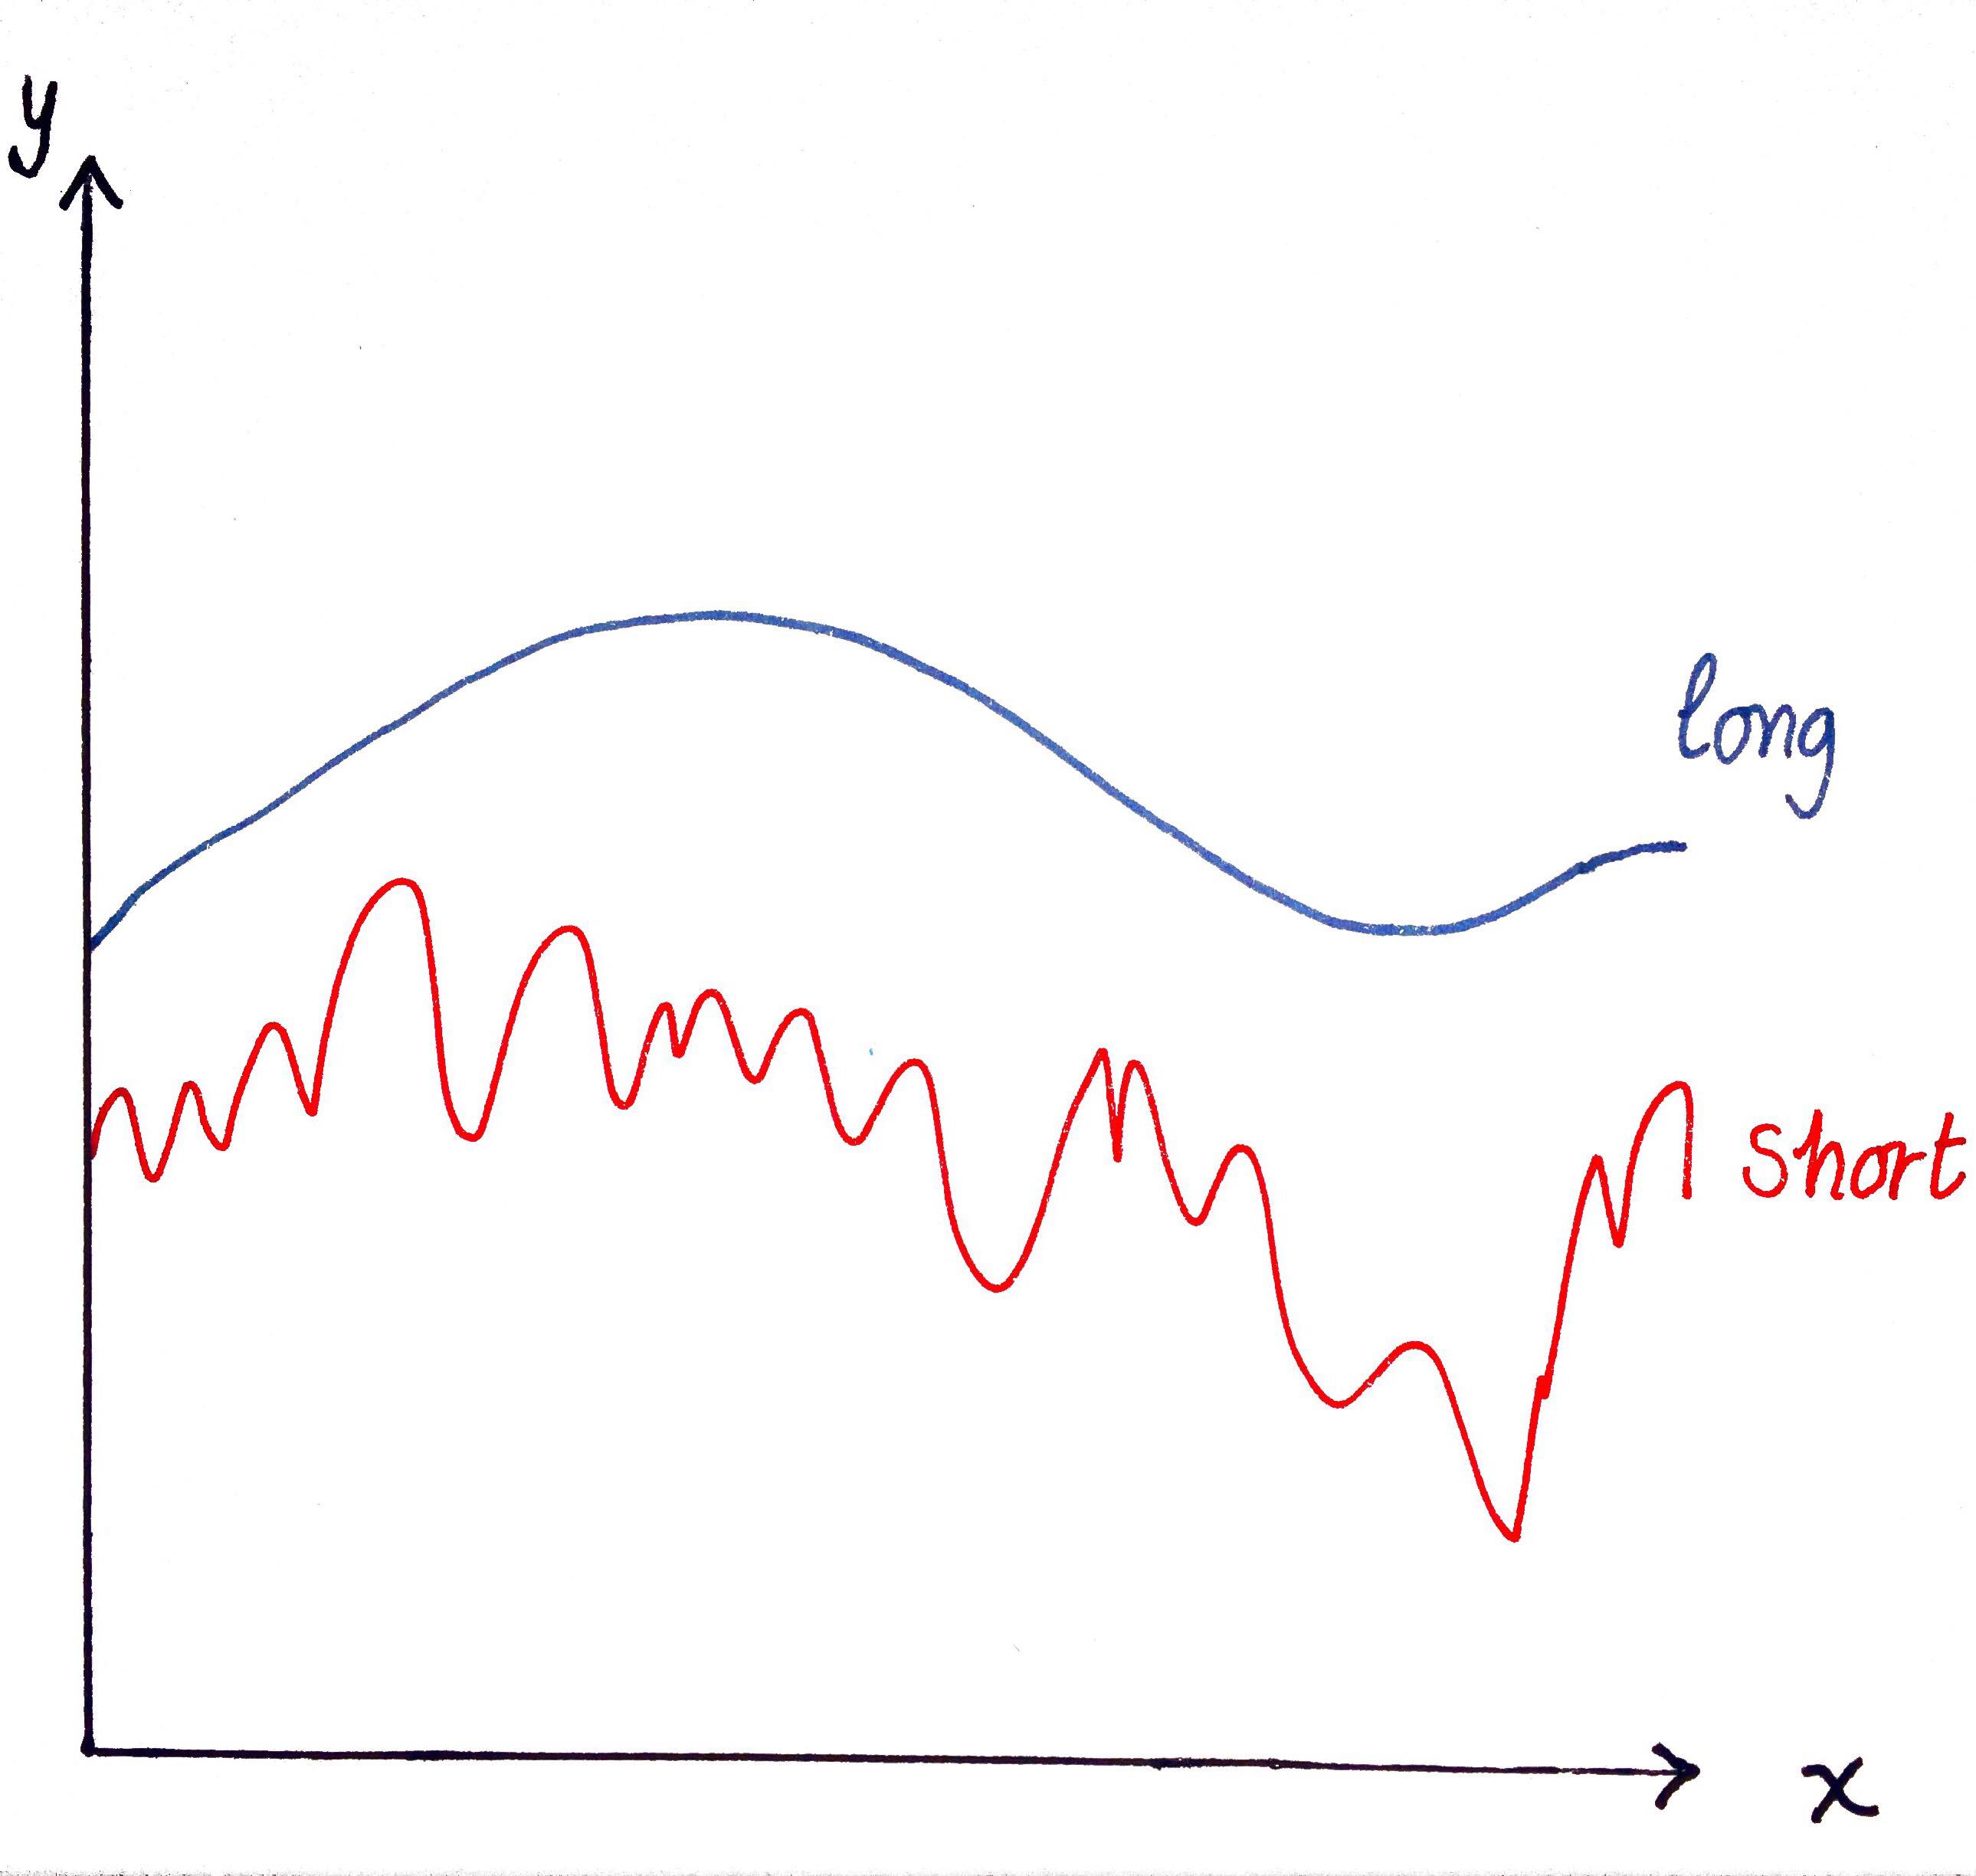
\includegraphics[scale=0.1]{GP_illustration_ell.jpg}
\caption{The effect of varying the length scale $\ell$. A large length scale (blue) gives a smooth, slowly varying function, while a small length scale (red) gives a more staccato, quickly varying function.}
\label{Fig:: gaussian process : ell variation example}
\end{figure}

The SE is implemented in \verb|scikit-learn| under the name radial basis function, and may be called in the following way for length scale $10$, with bounds on the length scale $[0.01, 100]$
\begin{lstlisting}
from sklearn.gaussian_process.kernels import RBF
rbf = RBF(length_scale=10, length_scale_bounds=(1e-2, 1e2))
\end{lstlisting}



\subsection{The Mat\'{e}rn Class }

The \textit{Mat\'{e}rn class of covariance functions} is given by
\begin{align}
k_{Mat\acute{e}rn} (r) = \frac{2^{1- \nu}}{\Gamma (\nu)} \Big( \frac{\sqrt{2 \nu} r	}{\ell} \Big)^{\nu} K_{\nu} \Big( \frac{\sqrt{2 \nu}r}{\ell} \Big),
\end{align}
where $\nu, \ell > 0$, and $K_{\nu}$ is a modified Bessel function. For $\nu \rightarrow \infty$ this becomes the SE. In the case of $\nu$ being half integer, $\nu = p + \frac{1}{2}$, the covariance function is simply the product of an exponential and a polynomial
\begin{align}
k_{\nu=p+\frac{1}{2}} = \exp \Big(- \frac{\sqrt{2 \nu} r	}{\ell} \Big) \frac{\Gamma(p+1)}{\Gamma(2p + 1)} \sum^p_{i=0} \frac{(p+i)!}{i!(p-i)!} \Big( \frac{\sqrt{8 \nu} r	}{\ell} \Big)^{p-i}.
\end{align}
In machine learning the two most common cases are for $\nu = 3/2$ and $\nu = 5/2$
\begin{align}
k_{\nu = 3/2}(r) &=  \Big(1 + \frac{\sqrt{3}r}{\ell} \Big) \exp \Big( -\frac{\sqrt{3}r}{\ell} \Big),\\
k_{\nu = 5/2}(r) &=  \Big(1 + \frac{\sqrt{5}r}{\ell}  + \frac{5r^2}{3 \ell^2}\Big) \exp \Big( -\frac{\sqrt{5}r}{\ell} \Big).
\end{align}

The Mat\'{e}rn kernel is considered more appropriate for physical processes \cite{rasmussen2006gaussian}, and may be called in \verb|scikit-learn| in the following way for length scale 10, length scale bounds $[0.01, 100]$ and $\nu = 3/2$
\begin{lstlisting}
from sklearn.gaussian_process.kernels import Matern
matern = Matern(length_scale=10, length_scale_bounds=(1e-2, 1e2), nu=1.5)
\end{lstlisting}

\subsubsection{Other Kernels}

There are other kernels which are not discussed here. Kernels can be multiplied and summed to form new kernels, making the space of possible kernels infinite. For further details see chapter 4 in \cite{rasmussen2006gaussian}.





\subsubsection{Hyperparameters}

Each kernel has a vector of hyperparameters, e.g. $\boldsymbol{\theta} = (\{M\}, \sigma^2_f, \sigma_n^2)$ for the radial basis function (RBF)
\begin{align}
k(\textbf{x}_i, \textbf{x}_j) = \sigma_f^2 \exp (- \frac{1}{2} (\textbf{x}_i - \textbf{x}_j))^T M (\textbf{x}_i - \textbf{x}_j) + \sigma_n^2 \delta_{ij}.
\end{align}
The matrix $M$ can have several forms, for example
\begin{align}
&M_1 = \ell^{-2} \mathbb{I} , &M_2 = \text{diag}(\vec{\ell})^{-2}.
\end{align}
Choosing $\vec{\ell}$ to be a vector in stead of a scalar can in many cases be useful, especially if the vector of features contain values of different scales, e.g. $\textbf{x} = (x_1, x_2)$ where $x_1 \in [0, 1]$ and $x_2 \in [200, 3000]$. The length scale can be set to a vector in \verb|scikit-learn| by giving the \verb|length_scale| parameter as a \verb|numpy| array of the same dimension as the feature vector $\textbf{x}$.



\section{Model Selection}

It becomes apparent that the choice of kernel and hyperparameters is important for the quality of the GP prediction. Model selection means finding the hyperparameters and kernel that best fit the data. In this section Bayesian model selection is quickly overviewed, and the log marginal likelihood and cross validation are considered for their ability to optimize the GP.

\subsection{Bayesian Model Selection}

A model has a set of model structures $\mathcal{H}_i$, hyperparameters $\boldsymbol{\theta}$ and parameters $\textbf{w}$. Feature selection is done at all levels in a hierarchical way, by finding the  posterior over \textit{parameters}, the posterior over \textit{hyperparameters} and the posterior for the \textit{model}. Here only the posterior over parameters is considered \cite{rasmussen2006gaussian},
\begin{align}
p(\textbf{w}| \textbf{y}, X, \boldsymbol{\theta}, \mathcal{H}_i) = \frac{p(\textbf{y} | X, \textbf{w}, \mathcal{H}_i) p(\textbf{w}|\boldsymbol{\theta}, \mathcal{H}_i)}{p(\textbf{y}|X, \boldsymbol{\theta}, \mathcal{H}_i)},
\end{align}
as it gives rise to the \textit{marginal likelihood} $p(\textbf{y}|X, \boldsymbol{\theta}, \mathcal{H}_i)$, given by 
\begin{align}
&p(\textbf{y}|X, \boldsymbol{\theta}, \mathcal{H}_i) = \int p(\textbf{y} | X, \textbf{w}, \mathcal{H}_i)p(\textbf{w}| \boldsymbol{\theta}, \mathcal{H}_i) d \textbf{w} & \text{(marginal likelihood)}.
\end{align}
Because of the complexity of integrals involved in model selection, it is common to maximize the marginal likelihood with respect to hyperparameters $\vec{\theta}$. This maximization is what distinguishes Bayesian model selection from other model selection schemes, as it incorporates a trade-off between model complexity and model fit. This means that a complex model will allow for several different kinds of models, but each of them will get a low probability. Meanwhile, simple models will only have a few possibilities, but each of these will have a large probability, see Fig. (\ref{Fig:: gaussian process : Marginal likelihood Rasmussen}).

\begin{figure}
\centering
\includegraphics[scale=0.4]{rasmussen_marginal_likelihood.png}
\caption{The marginal likelihood is the probability of the data, given the model. The number of data points $n$ and inputs $X$ are fixed. The horizontal axis represents an idealized set of all possible vectors of targets $\textbf{y}$. Since the marginal likelihood is a probability distribution it must normalize to unity. For a particular set $\textbf{y}$, indicated by the dotted gray line, the intermediate model is preferred to the simple and complex ones. Figure from \cite{rasmussen2006gaussian}.}
\label{Fig:: gaussian process : Marginal likelihood Rasmussen}
\end{figure}

%\begin{align}
%p( \boldsymbol{\theta}| \textbf{y}, X, \mathcal{H}_i) = \frac{p(\textbf{y} | X, \boldsymbol{\theta}, \mathcal{H}_i) p(\boldsymbol{\theta}| \mathcal{H}_i)}{p(\textbf{y}|X,  \mathcal{H}_i)}
%\end{align}
%\begin{align}
%p(\mathcal{H}_i| \textbf{y}, X) = \frac{p(\textbf{y} | X, \mathcal{H}_i) p( \mathcal{H}_i)}{p(\textbf{y}|X)}
%\end{align}

\subsection{Log Marginal Likelihood}

Gaussian process regression models with Gaussian noise have the wonderful trait of providing analytically tractable integrals for the marginal likelihood. The exact expression for the log marginal likelihood \footnote{The logarithm is used as the marginal likelihood varies rapidly.} can be shown to be \cite{rasmussen2006gaussian}
\begin{align}
\log p(\textbf{y}|X, \boldsymbol{\theta}) = - \frac{1}{2} \textbf{y}^T K_y^{-1} \textbf{y} - \frac{1}{2} \log |K_y| - \frac{n}{2} \log 2 \pi.
\end{align}
Each of the terms has an interpretation: $- \frac{1}{2} \textbf{y}^T K_y^{-1} \textbf{y}$ is the only term involving the data, and is therefore the data-fit; $-\frac{1}{2} \log |K_y|$ is the complexity penalty depending only on the covariance function and the inputs; and $- \frac{n}{2} \log 2 \pi$ is a normalization term. The marginal likelihood is conditioned on the hyperparameters of the covariance function $\vec{\theta}$, and the optimal parameters are found by maximizing. This requires the partial derivatives of the log marginal likelihood (LML)
\begin{align}
\frac{\partial}{\partial \theta_j}
 \log p(\textbf{y}|X, \boldsymbol{\theta}) = \frac{1}{2} \textbf{y}^T K^{-1} \frac{\partial K}{\partial \theta_j} K^{-1} \textbf{y} - \frac{1}{2} \text{tr} (K^{-1} \frac{\partial K}{\partial \theta_j}).
\end{align}
Computing the inverse of a matrix required here, $K^{-1}$, is computationally complex, and for $n$ training points goes as $\mathcal{O}(n^3)$. Once this is done, however, finding the partial derivatives only requires complexity $\mathcal{O}(n^2)$, and so gradient based optimizers are advantageous.

The LML can have several local optima, as seen in Fig. (\ref{Fig:: gaussian process : LML several local optima}). These correspond to different interpretations of the data. The rightmost optima in Fig. (\ref{Fig:: gaussian process : LML several local optima}) for example, favors a small length scale and smaller noise level. This means that it considers little of the data to be noise. The rightmost optima has a higher noise level, and allows for several large length scales, as it considers most of the data to be noise. Features with very high length scales are considered superfluous, as the function value depends little on them. Because of this type of complication, it might be wise to restart the optimizer a few times.

\begin{figure}
\centering
\includegraphics[scale=0.6]{/home/ingrid/Documents/Master/Programs/LML/plots/LML_two_local_maxima.pdf}
\caption{A contour plot of the log marginal likelihood with two local optima. The rightmost optima favours a short length scale and low noise, while the leftmost favors a high noise level and therefore several large length scales. Plot generated using scikit-learn.}
\label{Fig:: gaussian process : LML several local optima}
\end{figure}


\subsection{Cross Validation}

Cross validation is a means of monitoring the performance of a model. In k-fold validation this is done by dividing the data into $k$-subsets and using $k-1$ to train the model, and a single set to validate it. This is repeated $k$ times. Cross-validation requires a loss function, such as the mean relative deviance. 


%The error of an estimator can be divided into bias, variance and noise. The bias of an estimator is the average error for differing training sets, the variance is a measure of how sensitive the estimator is to varying data, and noise is a property of the data. High bias corresponds to a model that is too simple, i.e. that it considers much of the signal to be noise, while low bias corresponds to a model that is too complicated, i.e. that it fits the data perfectly but does not model the underlying function very well. 

Cross-validation can be used to plot learning curves, which is a tool to find out whether the model benefits from adding more data. The cross validation score uses the $R^2$ value, given by
\begin{align}
R^2 = 1 - \frac{\sum_{i=0}^{N-1} (y_i - \hat{y}_i)^2}{\sum_{i=0}^{N-1} (y_i - \bar{y})^2},
\end{align}
where $\hat{y}_i$ is the predicted value of the $i$th sample, $y_i$ is the true value and $\bar{y} = \frac{1}{N} \sum_{i = 0}^{N-1} y_i$ for $N$ samples. The learning curve plots the training score and validation score, which are used to find out if the model is \textit{overfitting} or \textit{underfitting}. \textit{Overfitting} means that the model is a perfect fit to the training data, but predicts poorly for test data. \textit{Underfitting} occurs when the model is not able to capture the underlying structure of the data. 

Examples of learning curves are shown in Fig. (\ref{Fig:: gaussian process : learning curves}) for Naive Bayes and SVM estimators. In a) both the training score and cross-validation score tend to a value below 1, which indicates underfitting. This model will not benefit from more data. The example in b) shows a training score of approximately 1, and a cross validation score that converges towards 1. This model could benefit from more data.

\begin{figure}
    \centering
    \begin{subfigure}[b]{0.45\textwidth}
        \includegraphics[width=\textwidth]{/home/ingrid/Documents/Master/ML/Benchmarks/learningcurve_2.pdf}
        \caption{Underfitting.}
        \label{fig:gull}
    \end{subfigure}
    \begin{subfigure}[b]{0.45\textwidth}
        \includegraphics[width=\textwidth]{/home/ingrid/Documents/Master/ML/Benchmarks/learningcurve.pdf}
        \caption{Well fit.}
        \label{fig:tiger}
    \end{subfigure}
\caption{Learning curves for two different estimators.}
\label{Fig:: gaussian process : learning curves}
\end{figure}



\subsection{Loss Functions}

In this project the main loss function used is the relative deviance. For true values $f_{true}$ and the GP prediction $f_{GP}$ this is given by
\begin{align}
\varepsilon = \frac{f_{true} - f_{GP}}{f_{true}}.
\end{align} 
The relative deviance is used because of the large span of the target values, ranging from about $10^{-30}$ to $10^9$.


\subsubsection{R-Factor}



\section{Distributed Gaussian Processes}

\subsection{Limitations of Gaussian Processes}

Problem because of $(K + \sigma_n^2 \mathbb{I})^{-1}$, means inverting an $n \times n$-matrix. Training and predicting limits of $\mathcal{O}(N^3)$ and $\mathcal{O}(N^2)$. Limit = $\mathcal{O}(10^4)$. Some solutions exist, but \textbf{no prediction of variance is given with p-o-e.}

\subsection{Product-of-Experts}

Divide data between experts. "The assumption of independent GP experts leads to a
block-diagonal approximation of the kernel matrix, which
(i) allows for efficient training and predicting (ii) can be
computed efficiently (time and memory) by parallelisation" \cite{deisenroth2015distributed}.

\begin{figure}
\centering
\includegraphics[scale=0.3]{product_of_experts.png}
\caption{From \cite{deisenroth2015distributed}.}
\end{figure}

Independence assumption
\begin{align}
p(\textbf{y} | \textbf{X}, \boldsymbol{\theta}) \approx \prod_{k=1}^M p_k(\textbf{y}^{(k)} | \textbf{X}^{(k)}, \boldsymbol{\theta}) 
\end{align}
\begin{align}
\log p(\textbf{y}^{(k)}|\textbf{X}^{(k)}, \boldsymbol{\theta}) = - \frac{1}{2} \textbf{y}^{(k)} (\textbf{K}_{\psi}^{(k)} + \sigma_{\varepsilon}^2 \textbf{I})^{-1}\textbf{y}^{(k)} - \frac{1}{2} \log
 |\textbf{K}_{\psi}^{(k)} + \sigma_{\varepsilon}^2 \textbf{I} |
\end{align}


\subsection{Algorithm}

\begin{align}
\mu_*^{rbcm} &= (\sigma_*^{rbcm})^2 \sum_k \beta_k \sigma_k^{-2} (\textbf{x}_*) \mu_k (\textbf{x}_*),\\
(\sigma_*^{rbcm})^{-2} &= \sum_{k=1}^M \beta_k \sigma_k^{-2} (\textbf{x}_*) + \big(1 - \sum_{k=1}^M \beta_k \big) \sigma_{**}^{-2}.
\end{align}
The posterior distribution for the test point $\textbf{x}_*$ is given by a Gaussian with mean and variance
\begin{align}
\mu (\textbf{x}_*) &= \textbf{k}_*^T (\textbf{K} + \sigma_{\epsilon}^2 \mathbb{I})^{-1} \textbf{y},\\
\sigma^2(\textbf{x}_*) &= k_{**} - \textbf{k}_*^T(\textbf{K} + \sigma_{\epsilon}^2 \mathbb{I})^{-1} \textbf{k}_*.
\end{align}




Plot of time from the article 

\begin{figure}
\centering
\includegraphics[scale=0.4]{DGP_times.png}
\caption{From \cite{deisenroth2015distributed}.}
\end{figure}

\subsection{Implementing the Algorithm}

\begin{algorithm}
 \KwData{$N_{experts}$ (number of experts), $X$ (inputs), \textbf{y} (targets), $k$ (covariance function/kernel), $\sigma_n^2$ (noise level), $\textbf{x}^*$ (test input), $\textbf{y}^*$ (test target)}
$X_{train}$, $X_{test}$, $y_{train}$, $y_{test}$ = train-test-split $(X, y)$ (scikit-learn) \;
$y = \log_{10} (y)$ \;
$n = \frac{\text{Number of data points}}{N_{experts}}$ \;
$subsets = array\_split (X_{train}, n)$ \;
$\mu_{rbcm} = []$, $\sigma_{rbcm} = []$  (empty lists to be filled later)\; 
\For {each expert}
{
$gp_{temporary} = GaussianProcessRegressor.fit(X_{expert}, y_{expert})$ \;
 \For {each $y^*$ in $\textbf{y}^*$}
 {
 $\mu_*,\sigma_*^2 = gp_{temporary}.predict(x^*)$ \;
 $\sigma_{**}^2 = k (x^*, x^*)$ \;
 (fill inn the values) \;
 $\boldsymbol{\mu}[\text{expert}][x^*] = \mu_*^2$ (mean value from this expert)\;
 $\boldsymbol{\sigma}^2[\text{expert}][x^*] = \sigma_*^2$ (variance from this expert)\;
 $\boldsymbol{\sigma}_{**}^2[\text{expert}][x^*] = \sigma_{**}^2$ (variance from initial kernel)
 }
}
 
\For {each expert}
{ 
\For {each $y_*$ in $\textbf{y}_*$}
{ $\mu_* = \boldsymbol{\mu}[\text{expert}][x_*]$ (retrieve relevant values)\;
$\sigma_*^2 = \boldsymbol{\sigma}^2[\text{expert}][x^*]$ \;
$\sigma_{**}^2 = \boldsymbol{\sigma}_{**}^2[\text{expert}][x^*]$ \; 
$\beta = \frac{1}{2} (\log (\sigma_{**}^2) - \log (\sigma_*^2))$ \;
$(\sigma_*^{rbcm})^{-2}[y_*] += \beta \sigma^{-2} + \big(\frac{1}{n_{experts}} - \beta \big) \sigma_{**}^{-2} $ }
 }  
\For {each expert}
{
\For {each $y_*$ in $\textbf{y}_*$}
 {
$\mu_* = \boldsymbol{\mu}[\text{expert}][x_*]$ (retrieve relevant values)\;
$\sigma_*^2 = \boldsymbol{\sigma}^2[\text{expert}][x^*]$ \;
$\sigma_{**}^2 = \boldsymbol{\sigma}_{**}^2[\text{expert}][x^*]$ \; 
$\beta = \frac{1}{2} (\log (\sigma_{**}^2) - \log (\sigma_*^2))$ \;
$\mu_*^{rbcm}[y_*] += (\sigma_*^{rbcm})^2 \beta \sigma^{-2}_* \mu_*$
 }
} 
$\epsilon = \frac{10^{\mu_{rbcm}} - 10^{y_{test}}}{10^{y_{test}}}$ (relative error)\;
\KwResult{Approximative distribution of $f_* = f(\textbf{x}_*)$ with mean $\mu^{rbcm}_*$ and variance $(\sigma^{rbcm}_*)^2$.}
 \caption{Algorithm for using rBCM on a single test point $\textbf{x}_*$. The $GaussianProcessRegressor.fit()$-function is a function in scikit-learn, that uses Algorithm (\ref{Alg:: GP}). }
\label{Alg:: DGP}
\end{algorithm}

\subsubsection{Parallelizing}

\subsection{Benchmark}



\bibliographystyle{plain}
\bibliography{dingsen_gaussian_processes}



\end{document}